\documentclass[a4paper, 14pt]{article}
\usepackage{pre}


\begin{document}
    % Оформление титульного листа
\begin{titlepage}
    \newpage
    
    \begin{center}
    МИНИСТЕРСТВО НАУКИ И ВЫСШЕГО ОБРАЗОВАНИЯ РОССИЙСКОЙ ФЕДЕРАЦИИ ФЕДЕРАЛЬНОЕ ГОСУДАРСТВЕННОЕ АВТОНОМНОЕ ОБРАЗОВАТЕЛЬНОЕ УЧРЕЖДЕНИЕ ВЫСШЕГО ОБРАЗОВАНИЯ НАЦИОНАЛЬНЫЙ ИССЛЕДОВАТЕЛЬСКИЙ ЯДЕРНЫЙ УНИВЕРСИТЕТ «МИФИ» \\
    \end{center}
    
    
    \vspace{2.5em} % Делаем вертикальный пробел в 3em
    
    \begin{center}
        \textsc{\textbf{Кафедра теоретической ядерной физики\\}}
    \end{center}
    \vspace{1em}
    \begin{center}
    \textsc{На правах рукописи\\} 
    \end{center}
    \begin{center}
        \textsc{\Large Широков Денис Дмитриевич\linebreak  \linebreak  \Large \textbf{ <<Численное решение уравнения теплопроводности с использованием локально-адаптивных сеток>>}}
    \end{center} 
    
    \vspace{1em}
    
    \begin{center}
    Выпускная квалификационная работа бакалавра \linebreak Направление подготовки 03.03.01 Прикладные математика и физика
    \end{center}
    
    \vspace{1em}
    
   
    \newbox{\lbox}
    \savebox{\lbox}{\hbox{Широков Денис Дмитриевич}}
    \newlength{\maxl}
    \setlength{\maxl}{\wd\lbox}
    \hfill\parbox{9cm}{
    \hspace*{1.5cm}\hspace*{-3cm}Выпускная квалификационная\\ \hspace*{1.5cm}\hspace*{-3cm}работа защищена\\ 
    
    \hspace*{1.5cm}\hspace*{-3cm}<<\rule{1.5em}{1pt}>>\hbox to\maxl{\rule{6em}{1pt}2021 г.\hfill}\\
    
    \hspace*{1.5cm}\hspace*{-3cm}Оценка \hbox to\maxl{\rule{7em}{1pt}\hfill}\\
    
    \hspace*{1.5cm}\hspace*{-3cm}Секретарь ГЭК 
    \hbox to\maxl{\rule{5em}{1pt} Корнеев Ф.А.\hfill}\hfill\\  
    \hspace*{7.0cm}\hspace*{-3cm}к.ф.-м.н., доцент\hfill\\
    
    }
    
    

    
    
    \vspace{\fill}
    
    \begin{center}
    \textbf{Москва}\\
    \today
    \end{center}

\end{titlepage}

    % Оформление титульного листа
\begin{titlepage}
    \newpage
    
    \vspace{3em} % Делаем вертикальный пробел в 3em
    
   
    \begin{center}
        \textsc{ \textbf{Пояснительная записка\linebreak к бакалаврской дипломной работе: \linebreak  \Large <<Численное решение уравнения теплопроводности с использованием локально-адаптивных сеток>>}}
    \end{center} 

    
    \vspace{5em}
    
   
    \newbox{\lbox}
    \savebox{\lbox}{\hbox{Широков Денис Дмитриевич}}
    
    \setlength{\maxl}{\wd\lbox}
    \hfill\parbox{12cm}{
    \hspace*{1cm}\hspace*{-1cm}Студент\hfill\hbox to\maxl{\rule{5em}{1pt} Широков Д.Д.\hfill}\\
    
    \hspace*{1cm}\hspace*{-1cm}Научный руководитель\hfill\\
    \hspace*{1cm}\hspace*{-1cm}к.ф.-м.н.\hfill\hbox to\maxl{\rule{5em}{1pt} Кучугов П.А.\hfill}\\ \\
    \hspace*{1cm}\hspace*{-1cm}Рецензент\hfill\\
    \hspace*{1cm}\hspace*{-1cm}к.ф.-м.н.\hfill\hbox to\maxl{\rule{5em}{1pt} Ладонкина М.Е. \hfill}\\ \\ 
    \hspace*{1cm}\hspace*{-1cm}Заведующий кафедрой \hfill\\
    \hspace*{1cm}\hspace*{-1cm}к.ф.-м.н.\hfill\hbox to\maxl{\rule{5em}{1pt} Муравьев С.Е. \hfill}\\ \\ 
    
    }
    
   
    
    


\end{titlepage}


    % Аннотация
    \section*{Аннотация}
    В работе проведён подробный анализ численного метода разностных схем решения уравнения теплопроводности, исследуются преимущества и недостатки использования равномерных статических сеток в случае квазилинейных уравнений с существенно различающимися масштабами (как пространственными, так и временными) физических процессов.
Разработано программное обеспечение, реализующее рассмотренные схемы численного решения, проверены описанные особенности каждой из схем.
Показана необходимость использования сеток с локальным измельчением, подстраивающихся под особенности решения.
Описаны некоторые теоретические основы данного метода.
Реализован в виде программного кода соответствующий алгоритм, работоспособность которого проверена на нескольких тестовых задачах.
Показаны преимущества использования блочных локально-адаптивных сеток по сравнению с использованием равномерных статических.
    \newpage

    % Содержание
    \tableofcontents
    \newpage

    % Введение
    \section*{Введение}
    \addcontentsline{toc}{section}{Введение}
    Большинство моделей классической физики, таких как гидрогазодинамика, описываются начально-краевыми задачами для дифференциальных уравнений в частных производных второго порядка\cite{ТихоновСамарский, ЛандауГидродинамика}.
Нахождение аналитического решения таких задач представляется возможным только в случае простых, канонических областей (таких как круг, шар, прямоугольник), простых начальных и граничных условий, а также в случае линейных уравнений, описывающих простые физические процессы.

На практике же часто возникают нелинейные задачи, поставленные в областях сложной формы.
Например, задача лазерного термоядерного синтеза (ЛТС), идя которой заключается в быстром нагреве и сжатии термоядерного топлива до температур и плотностей, необходимых для осуществления быстрого и эффективного протекания термоядерных реакций инерциально удерживаемой плазмы.
Процессы распространения тепла в такой системе будут описываться нелинейным уравнением теплопроводности.
Нелинейное уравнение теплопроводности также возникает в, например, задачах о самофокусировки световых пучков в нелинейных средах, эффекте $T$--слоя в низкотемпературной плазме, проблемы безударного сжатия; вообще с необходимостью в любой задаче, в которой присутствуют процессы самопроизвольного нарушения симметрии с понижением её степени \cite{ГалактионовКвазилинейное} 

Любой численный метод приближённого решения таких задач использует дискретизацию (то есть переход от бесконечномерного функционального пространства к конечномерному пространству).
Один из основных методов~--- \emph{метод конечных разностей}.
Его основа заключается в том, что исходная непрерывная задача в области $G \subset \mathbb{R}^n$ сводится к \emph{семейству разностных задач}~--- системам конечного числа линейных (в общем случае~--- нелинейных) уравнений на т.н. \emph{разностные функции}~--- функции, заданные на конечном числе точек (именуемое \emph{сеткой}), и принимающие значения (приближённые значения решения) на конечном числе точек.
Такие задачи решаются алгоритмически и тем самым могут быть программно реализованы на современных ЭВМ.
Более подробно метод описан в разделе~\ref{sec:MainDiffSchemes}.

Принципиальная возможность применения тех или иных алгоритмов основывается на вопросе об их сходимости, точности и устойчивости.
Так, в работе \cite{СамарскийТеорияРазностныхСхем} даётся обширное описание алгоритмов решения задач на \emph{статических} сетках, исследуются вопросы устойчивости и скорости сходимости.
Более подробное исследование тех же вопросов в случае \emph{неравномерных статических сеток} дан в работе \cite{СамарскийНеравномерныеСетки}.

Как уже отмечалось, в прикладных задачах приходится сталкиваться с квазилинейными уравнениями теплопроводности:
\begin{equation*}
    \frac{\partial u}{\partial t} =
    \sum\limits_{\alpha = 1}^{p} \frac{\partial }{\partial x_{\alpha}} \left[ 
        k_{\alpha}(u) \frac{\partial u}{\partial x_{\alpha}}
     \right]
\end{equation*}
Проблема использования \emph{статических} сеток, то есть сеток, не меняющихся на протяжении всего алгоритмического процесса поиска решения, связана со следующим обстоятельством.
В статьях \cite{ЗельдовичРазрывы, ЕщёРазрывы} показано, что одномерное уравнение теплопроводности в случае зависящего от температуры коэффициента теплопроводности имеет решения, производные которых разрывны в точках обращения в нуль решения $u(x, t)$, при этом поток тепла $k(u) \frac{\partial u}{\partial x}$~--- непрерывен, то есть существует фронт температуры, который, как показано в \cite{ЕщёЕщёРазрывы}, распространяется с конечной скоростью.
Эти \glqq проблемные точки решения\grqq оказываются сильно локализованными:
если для численного решения использовать достаточно грубые сетки, то основные ошибки в приближённом решении будут локализованны именно в окрестностях этих точек.
Конечно, можно использовать более мелкий шаг сетки и улучшить точность решения, ибо, как предсказывает теория \cite{СамарскийТеорияРазностныхСхем}, приближённое решение должно сходится к точному при стремлении шага сетки к нулю.

Однако даже на мощных вычислитльных системах расчёт сложных трёхмерных задач со сложной пространственной геометрией требует огромного числа точек сетки, что значительно увеличивает используемую память и расчётное время \cite{АфендиковЛАД}.
Более того, точность решения в области особенностей \emph{существенно} влияет на точность решения во всей остальной области.
Поэтому хотя бы для получения приемлемой кратины решения в целом на всей области без точного учёта особенностей неизбежно приходится сильно измельчать сетку.
Учитывая, что в подобластях гладкого поведения решения просто нет необходимости измельчать сетку настолько сильно, заключаем, что использование классических алгоритмов приводит к тому, что большая часть компьютерных вычислений производится напрасно.

Поэтому для данного класса гидродинамических проблем с локализованными особенностями разрабатывались специальные методы \emph{локально\hyp адаптивных сеток} (\emph{Adaptive mesh refinement}), учитывающие разномасштабное поведение решения.
Например, в работе \cite{СамарскийАдаптивные} предлагалось использовать адаптивную сетку, построение которой производится с помощью соответствующего преобразования координат.
Конкретный вид преобразования задаётся с помощью некоторой функции $Q$, вид которой определяется особенностями решения исследуемой задачи.
Т.к. вид функции $Q$ выбирался вручную в завимимости от конкретной задачи, этот метод не обладал достаточной автономностью.
Многие методы были основаны на геометрической адаптации рассчётных сеток, что, в свою очередь, приводит к трудностям реализации на ЭВМ, поскольку неструктурированные сетки порождают нерегулярный доступ к памяти.
С учётом современного развития массивно-параллельных архитектур процессоров с большим числом ядер, эффективность работы которых зависит в первую очередь от упорядоченности обращений в память, производительность методов с неструктурированными сетками оказывается неудовлетворительной.

\emph{Метод структурированных адаптивных сеток (Block-structured adaptive mesh refinement)} был представлен в работах \cite{berger1982adaptive, berger1989local} применительно к уравнениям гиперболического типа.
Преимущества метода в:
\begin{itemize}
    \item использовании простых прямоугольных областей определённого размещения, удобных для реализации на компьютере
    \item возможности использования архитектуры параллельных вычислений
    \item использовании точно таких же разностных схем, как и для статических декартовых сеток (с некоторыми алгоритмическими модификациями)
\end{itemize}.

\textbf{Целью данной работы} является изучение метода стрктурированных декартовых локально-адаптивных сеток применительно к задачам для уравнения теплопроводности, программная реализация данного метода, сравнение со статическими аналогами.

В разделе \ref{sec:MainDiffSchemes} вводятся основные математические формулировки разностных задач.
В разделе \ref{sec:StaticGrid} описываются алгоритмы решения задач на статических сетках (которые в последствии непосредственно используются при решении методом адаптивных сеток), приводятся примеры решения модельных задач.
В разделе \ref{sec:LAG} приводится описание метода, программной реализации и результатов решения модельных задач.

    % Основные понятия теории разностных схем
    \section{Основные понятия теории разностных схем}\label{sec:MainDiffSchemes}
    Математическая формулировка физических задач, описанных во введении имеет вид:
\begin{equation}\label{eq:InitialProblem}
    \begin{cases}
        L[u](x) = f(x), & x = (x_1, \ldots, x_n)^{T} \in G \subset \mathbb{R}^n\\
        \Gamma[u](x) = \mu(x), & x \in \partial G
    \end{cases}, 
\end{equation}
где 
\begin{itemize}
    \item $L$~--- дифференциальный оператор уравнения;
    \item $\Gamma$~--- оператор начально-краевых условий (в общем случае также дифференциальный);
    \item $f$, $\mu$~--- заданные функции.
\end{itemize}
Решения исходной задачи~--- функции $u(x)$ непрерывного аргумента $x \in G$, являются элементами некоторого функционального пространства $H_0$ с нормой $\norm{\cdot}$.
В методе конечных разностей область $G$ заменяется на некоторое дискретное множество точек $\omega_h$, именуемое \emph{сеткой}, а функциональное пространство $H_0$ заменяется на $H_h$~--- гильбертово пространство сеточных функций ${y_h : G \supset \omega_h \rightarrow \mathbb{R}}$, где $h$~--- некоторый параметр, характеризующий сетку $\omega_h$ в области $G$.
Например, равномерная статическая сетка:
\begin{equation*}
    \omega_h = \{x = (x_1, \ldots, x_n) \in G \mid x_i = h_i \cdot k,\,\, k = 0, 1, \ldots, N_i\,\, i = 1, \ldots, n\}
\end{equation*}
Получив приближённое решение задачи $y_h$, необходимо оценивать степень \glqq близости\grqq к решению исходной задачи $u(x)$.
$y_h$~и~$u$ являются элементами разных функциональных пространств, поэтому для оценивания близости в работе используется проекционный метод: пространство $H_0$ отображается (проектируется) на пространство $H_h$ оператором $\mathcal{P}$:
\begin{equation*}
    \mathcal{P}_h \colon H_0 \ni u \mapsto u_h \in H_h.
\end{equation*}
Простейший выбор: ограничение $u$ на сетку $\omega_h$:
\begin{equation*}
    u_h(x) := u(x),\quad x \in \omega_h \subset G
\end{equation*}
Иногда пользуются \glqq более равномерным\grqq способом ограничения с усреднением по окрестности узла:
\begin{equation*}
    u_h(x) := \frac{1}{2h} \int_{x - h}^{x + h} u(x') dx'
\end{equation*}
Тогда близость приближённого решения $y_h$ и исходного решения $u$ оценивается по норме $\norm{\cdot}_{h}$ пространства $H_h$:
\begin{equation*}
    e = \norm{y_h - u_h}_{h},
\end{equation*}
при этом требуется, чтобы она аппроксимировала норму $\norm{\cdot}_{0}$ в слудеющем смысле\cite{СамарскийТеорияРазностныхСхем}:
\begin{equation*}
    \lim\limits_{h \rightarrow 0} \norm{u_h}_h = \norm{u}_{0}
\end{equation*}
В работе используется норма
$
    \norm{y}_{h} = \sqrt{
        \sum_{i=1}^{N} hy_i^2
    }
$.
Исходному дифференциальному оператору $L$ ставится в соответствие \emph{разностный оператор} $L_h$:
\begin{equation*}
    L_h[v] (x) = \sum_{x' \in T(x)} A_h(x, x') v(x'),
\end{equation*}
где $T(x)$~--- некоторое множество узлов сетки, называемое \emph{шаблоном}.
Например, двумерный оператор Лапласа $L = \Delta$ на двумерной равномерной сетке можно аппроксимировать, используя шаблон \glqq крест\grqq (\seefigref{fig:cross}):
\begin{equation*}
    \Delta u(x) = \frac{\partial^2 u}{\partial x_1^2} + \frac{\partial^2 u}{\partial x_2^2} \mapsto 
    \frac{u_{i+1}^{j} - 2u_{i}^{j} + u_{i-1}^j}{h_1^2} +
    \frac{u_i^{j + 1} - 2u_i^{j} + u_i^{j-1}}{h_2^2}, 
\end{equation*}
где $u_i^j = u({x_1}_i, {x_2}_j),\quad ({x_1}_i, {x_2}_j) \in \omega_h$.
\begin{figure}
    \centering
    \begin{tikzpicture}
        \filldraw[black] (0, 0) circle(2pt) node[anchor=south west] {$(x_1, x_2)$};
        \draw (-2.5, 0) node[anchor=north] {$(x_1 - h_1, x_2)$} -- (2.5, 0) node[anchor=north] {$(x_1 + h_1, x_2)$};
        \filldraw[black] (-2.5, 0) circle(2pt);
        \filldraw[black] (2.5, 0) circle(2pt);
        \filldraw[black] (0, -2.5) circle(2pt);
        \filldraw[black] (0, 2.5) circle(2pt);
        \draw (0, -2.5) node[anchor=north] {$(x_1, x_2 - h_2)$} -- (0, 2.5) node[anchor=south] {$(x_1, x_2 + h_2)$};
    \end{tikzpicture}
    \caption{Шаблон \glqq Крест\grqq}
    \label{fig:cross}
\end{figure}
Погрешность аппроксимации оператора $L$ разностным оператором $L_h$ определяется как сеточная функция $\psi_h = L_h[u_h] - (L[u])_h, u \in H_0$.
Если $\norm{\psi_h} = O(|h|^m)$, то говорят, что оператор $L_h$ аппроксимирует оператор $L$ с порядком $m$.
Если $\psi(x) = O(h^m), m$, то говорят, что оператор $L_h$ аппроксимирует оператор $L$ в точке $x$ с порядком $m$.

Теперь сформулируем непосредственно то, что называется \emph{разностной схемой}, алгоритмы решения которой и реализуются на компьютере.
Исходной задаче \eqref{eq:InitialProblem} ставится в соответствие семейство разностных задач, зависящих от параметра $h$, называемое разностной схемой:
\begin{equation*}
    \left\{ 
        \begin{cases}
            L_h [y_h] = \phi_h, & x \in \omega_h\\
            l_h [y_h] = \chi_h, & x \in \gamma_h
        \end{cases}
     \right\}_h,\quad \phi_h = \mathcal{P}_h[f], \chi_h = \mathcal{P}_h[\mu]
\end{equation*}
Под погрешностью разностной схемы понимается $z_h = y_h - u_h$, где $u_h = \mathcal{P}_h u$~--- проекция решения исходной задачи на $H_0$. 
Решения разностной задачи сходится к решению исходной задачи, если 
\begin{equation*}
    \norm{z_h}_{h} \rightarrow 0 \text{ при } |h| \rightarrow 0
\end{equation*}
Введём также понятие устойчивости схемы.
Разностная схема называется устойчивой (корректной, сходящейся), если
$
    \exists h_0 > 0 : \forall h(|h| \le h_0) \Rightarrow
$
\begin{equation*}
    \begin{aligned}
        &1. \forall \phi \in H_h \quad \exists! y_h\text{--- решение};\\
        &2. \exists M > 0 : \forall \phi_h, \tilde{\phi}_h \norm{y_h - \tilde{y}_h} \le M \norm{\phi_h - \tilde{\phi}_h}
    \end{aligned}
\end{equation*}

На этом только лишь математическая сторона вопроса формулирования проблемы завершена. 
Дальнейшие шаги по исследованию разностной схемы опираются на конкретный выбор множества сеток $\left\{ \omega_h \right\}$ и аппроксимирующего оператора $L_h$, выбор которого, в свою очередь, существенно зависит от некоторых вопросов реализации получаемого алгоритма на компьютере.







% например, в случае квазилинейного уравнения теплопроводности
% $
%     L = \frac{\partial }{\partial t} - 
%     \sum\limits_{i = 1}^{n} \frac{\partial }{\partial x_i} \left( 
%         k(x) \frac{\partial u}{\partial x_i}
%      \right)
% $;

% Сетки и сеточные функции
% Пусть $H_0$~--- некоторое функциональное пространство функций $u(x)$ непрерывного аргумента $x \in G$ с нормой $\|\cdot\|_0$.
% В методе конечных разностей область $\bar{G}$ изменения аргумента $x$ заменяется сеткой $\bar{\omega}_h$~--- конечным множеством точек $x_i \in \bar{G}$,
% а функциональное пространство $H_0$ заменяется на $H_h$~--- гильбертово пространство сеточных функций $y_h(x)$, определённых на сетке $\bar{\omega}_h$ с нормой $\|\cdot\|_h$.
% Обычно будем пользоваться нормой $\|y\|_h = \left( \sum\limits_{i = 1}^{N} h y_i^2 \right)^{1/2}$
% Функции $y_h(x) \in H_h$~--- численные решения, аппроксимации исходных решений $u(x) \in H_0$.
% Соответственно, основной интерес теории приближённых методов представляет \textbf{оценка близости} $y_h$ к $u$.
% Эти два вектора являются элементами разных пространств. Их близость описываем следующим образом:

% $\mathcal{P}_h: H_0 \rightarrow H_h,\quad u \mapsto u_h: u_h(x) = u(x), x \in \bar{\omega}_h$.
% Тогда близость $u_h$ и $y_h$ характеризуется числом $\|y_h - u_h\|_h$.

% Условие согласования норм в $H_h$ и $H_0$:
% $\lim\limits_{h \rightarrow 0} \|u_h\|_h = \| u\|_0$, или другими словами "норма $\|\cdot\|_h$ аппроксимирует норму $\|\cdot\|_0$"


% Разностная аппроксимация дифференциальных операторов

% Пусть $L$~--- линейный дифференциальный оператор, $\mathcal{D}(L) = H_0$, $\quad Ш(x) \subset \bar{\omega}_h$~--- некоторое множество узлов сетки

% \textbf{Опр.} $L_h v_h (x) = L_h v_h(x) = \sum\limits_{\xi \in Ш(x)} A_h(x, \xi) v_n (\xi)$~--- разностный оператор, разностная аппроксимация оператора $L$

% \textbf{Опр.} $\psi(x) = L_h v(x) - L v(x)$~--- локальная погрешность разностной аппроксимации $Lv$ в точке $x$.

% \textbf{Опр.} $L_h$ аппроксимирует $L$ с порядком $ m > 0$ в точке $x$, если $\psi(x) = L_h v(x) - Lv(x) = O(h^m)$

% \textbf{Опр.} Погрешность аппроксимации оператора $L$ разностным оператором $L_h$~--- это сеточная функция
% $\psi_h = L_h v_h - (Lv)_h, \quad (Lv)_h = \mathcal{P}_h (Lv), \quad v \in H_0$

% \textbf{Опр.} Разностный оператор $L_h$ аппроксимирует дифференциальный оператор $L$ с порядком $m>0$, если
% $$
%     \| \psi_h \| = \| L_h v_h - (Lv)_h \|_h = O(|h|^m)
% $$

% Общее утверждение, касательно аппроксимации дифференциальных операторов разностными таково, что:
% * погрешность аппроксимации зависит от используемого шаблона, причём можно достичь любого порядка локальной аппроксимации повышением кол-ва узлов шаблона (однако ухудшается качество операторов)
% * исследование локальной аппроксимации может оказаться недостаточным для суждения о порядке разностной аппроксимации на сетке и тем самым для суждения о качестве разностного оператора
% * рассмотрение разностной аппроксимации на решении дифференциального уравнения может использоваться для повышения порядка аппроксимации


% Постановка разностных задач.

% $G\subset \mathbb{R}^n$, $\partial G = \Gamma$, $L, l$~--- линейные дифференциальные операторы, $\mathcal{D}(L) = H_0$, $\mathcal{D}(l) = H_0$. 
% Исохдной задаче
% $$
%     \begin{cases}
%         Lu(x) = f(x), & x \in G\\
%         lu(x) = \mu (x), & x \in \Gamma
%     \end{cases}
% $$
% ставится в соответствие *семейство разностных задач*, зависящих от параметра $h$, называемое *разностной схемой*:
% $$
%     \left\{ 
%         \begin{cases}
%             L_h y_h = \varphi_h, & x \in \omega_h\\
%             l_h y_h = \chi_h, & x \in \gamma_h
%         \end{cases}
%         \right\}_h
% $$

% \textbf{Опр.} Погрешность разностной схемы $z_h = y_h - u_h$, где $y_h$~--- решение разностной задачи, а $u_h = \mathcal{P}_h u$ проекция решения исходной задачи на $H_0$.

% \textbf{Опр.} Погрешность аппроксимации для уравнения $L_h y_h = \varphi_h$ на решении $u(x)$ уравнения $Lu = f$:
% $$
%     \psi_h = L_h z_h = \varphi_h - L_h u_h
% $$
% погрешность аппроксимации для условия $l_h y_h = \chi_h$ на решении $u(x)$ исходной задачи:
% $$
%     \nu_h = l_h z_h = \chi_h - l_h u_h
% $$

% \textbf{Опр.} Решение разностной задачи *сходится к решению исходной задачи*, если 
% $$
%     \| z_h\|_h = \|y_h - u_h \|_h \rightarrow 0 \quad  |h| \rightarrow 0
% $$

% \textbf{Опр.} Разностная схема *сходится со скоростью* $O(|h|^m)$ (*имеет $m$-ый порядок точности*), если 
% $$
%     \| z_h \|_h = \| y_h - u_h \|_h = O(|h|^m), \quad |h| \rightarrow 0
% $$

% \textbf{Опр.} Разностная схема обладает $n$-ым порядком аппроксимации, если
% $$
%     \| \psi_h \|_h = O(|h|^n),\quad \| \nu_h \|_h = O(|h|^n)
% $$

% \textbf{Опр.} Разностная схема называется корректной (устойчивой, сходящейся), если
% $\exists h_0 > 0 : \forall h (|h| \leqslant h_0) \Rightarrow$
% 1. $\forall \varphi \in \tilde{H}_h \,\, \exists ! y_h$~--- решение;
% 2. $\exists M > 0 : \forall \varphi_h, \tilde{\varphi}_h \quad \| y_h - \tilde{y}_h \| \leqslant M \| \varphi_h - \tilde{\varphi}_h \|$

% **Утв.** Если схема устойчива и аппроксимирует исходную, т.е. $\| \psi_h \|_h = O(|h|^n)$, то она сходится, причём порядок сходимости совпадает с порядком аппроксимации.

    % Разностные схемы на статических сетках
    \section{Разностные схемы на статических сетках}\label{sec:StaticGrid}
        % Общие замечания
        Большинство моделей классической физики, таких как гидрогазодинамика, описываются начально-краевыми задачами для дифференциальных уравнений в частных производных второго порядка\cite{ТихоновСамарский, ЛандауГидродинамика}.
Нахождение аналитического решения таких задач представляется возможным только в случае простых, канонических областей (таких как круг, шар, прямоугольник), простых начальных и граничных условий, а также в случае линейных уравнений, описывающих простые физические процессы.

На практике же часто возникают нелинейные задачи, поставленные в областях сложной формы.
Например, задача лазерного термоядерного синтеза (ЛТС), идя которой заключается в быстром нагреве и сжатии термоядерного топлива до температур и плотностей, необходимых для осуществления быстрого и эффективного протекания термоядерных реакций инерциально удерживаемой плазмы.
Процессы распространения тепла в такой системе будут описываться нелинейным уравнением теплопроводности.
Нелинейное уравнение теплопроводности также возникает в, например, задачах о самофокусировки световых пучков в нелинейных средах, эффекте $T$--слоя в низкотемпературной плазме, проблемы безударного сжатия; вообще с необходимостью в любой задаче, в которой присутствуют процессы самопроизвольного нарушения симметрии с понижением её степени \cite{ГалактионовКвазилинейное} 

Любой численный метод приближённого решения таких задач использует дискретизацию (то есть переход от бесконечномерного функционального пространства к конечномерному пространству).
Один из основных методов~--- \emph{метод конечных разностей}.
Его основа заключается в том, что исходная непрерывная задача в области $G \subset \mathbb{R}^n$ сводится к \emph{семейству разностных задач}~--- системам конечного числа линейных (в общем случае~--- нелинейных) уравнений на т.н. \emph{разностные функции}~--- функции, заданные на конечном числе точек (именуемое \emph{сеткой}), и принимающие значения (приближённые значения решения) на конечном числе точек.
Такие задачи решаются алгоритмически и тем самым могут быть программно реализованы на современных ЭВМ.
Более подробно метод описан в разделе~\ref{sec:MainDiffSchemes}.

Принципиальная возможность применения тех или иных алгоритмов основывается на вопросе об их сходимости, точности и устойчивости.
Так, в работе \cite{СамарскийТеорияРазностныхСхем} даётся обширное описание алгоритмов решения задач на \emph{статических} сетках, исследуются вопросы устойчивости и скорости сходимости.
Более подробное исследование тех же вопросов в случае \emph{неравномерных статических сеток} дан в работе \cite{СамарскийНеравномерныеСетки}.

Как уже отмечалось, в прикладных задачах приходится сталкиваться с квазилинейными уравнениями теплопроводности:
\begin{equation*}
    \frac{\partial u}{\partial t} =
    \sum\limits_{\alpha = 1}^{p} \frac{\partial }{\partial x_{\alpha}} \left[ 
        k_{\alpha}(u) \frac{\partial u}{\partial x_{\alpha}}
     \right]
\end{equation*}
Проблема использования \emph{статических} сеток, то есть сеток, не меняющихся на протяжении всего алгоритмического процесса поиска решения, связана со следующим обстоятельством.
В статьях \cite{ЗельдовичРазрывы, ЕщёРазрывы} показано, что одномерное уравнение теплопроводности в случае зависящего от температуры коэффициента теплопроводности имеет решения, производные которых разрывны в точках обращения в нуль решения $u(x, t)$, при этом поток тепла $k(u) \frac{\partial u}{\partial x}$~--- непрерывен, то есть существует фронт температуры, который, как показано в \cite{ЕщёЕщёРазрывы}, распространяется с конечной скоростью.
Эти \glqq проблемные точки решения\grqq оказываются сильно локализованными:
если для численного решения использовать достаточно грубые сетки, то основные ошибки в приближённом решении будут локализованны именно в окрестностях этих точек.
Конечно, можно использовать более мелкий шаг сетки и улучшить точность решения, ибо, как предсказывает теория \cite{СамарскийТеорияРазностныхСхем}, приближённое решение должно сходится к точному при стремлении шага сетки к нулю.

Однако даже на мощных вычислитльных системах расчёт сложных трёхмерных задач со сложной пространственной геометрией требует огромного числа точек сетки, что значительно увеличивает используемую память и расчётное время \cite{АфендиковЛАД}.
Более того, точность решения в области особенностей \emph{существенно} влияет на точность решения во всей остальной области.
Поэтому хотя бы для получения приемлемой кратины решения в целом на всей области без точного учёта особенностей неизбежно приходится сильно измельчать сетку.
Учитывая, что в подобластях гладкого поведения решения просто нет необходимости измельчать сетку настолько сильно, заключаем, что использование классических алгоритмов приводит к тому, что большая часть компьютерных вычислений производится напрасно.

Поэтому для данного класса гидродинамических проблем с локализованными особенностями разрабатывались специальные методы \emph{локально\hyp адаптивных сеток} (\emph{Adaptive mesh refinement}), учитывающие разномасштабное поведение решения.
Например, в работе \cite{СамарскийАдаптивные} предлагалось использовать адаптивную сетку, построение которой производится с помощью соответствующего преобразования координат.
Конкретный вид преобразования задаётся с помощью некоторой функции $Q$, вид которой определяется особенностями решения исследуемой задачи.
Т.к. вид функции $Q$ выбирался вручную в завимимости от конкретной задачи, этот метод не обладал достаточной автономностью.
Многие методы были основаны на геометрической адаптации рассчётных сеток, что, в свою очередь, приводит к трудностям реализации на ЭВМ, поскольку неструктурированные сетки порождают нерегулярный доступ к памяти.
С учётом современного развития массивно-параллельных архитектур процессоров с большим числом ядер, эффективность работы которых зависит в первую очередь от упорядоченности обращений в память, производительность методов с неструктурированными сетками оказывается неудовлетворительной.

\emph{Метод структурированных адаптивных сеток (Block-structured adaptive mesh refinement)} был представлен в работах \cite{berger1982adaptive, berger1989local} применительно к уравнениям гиперболического типа.
Преимущества метода в:
\begin{itemize}
    \item использовании простых прямоугольных областей определённого размещения, удобных для реализации на компьютере
    \item возможности использования архитектуры параллельных вычислений
    \item использовании точно таких же разностных схем, как и для статических декартовых сеток (с некоторыми алгоритмическими модификациями)
\end{itemize}.

\textbf{Целью данной работы} является изучение метода стрктурированных декартовых локально-адаптивных сеток применительно к задачам для уравнения теплопроводности, программная реализация данного метода, сравнение со статическими аналогами.

В разделе \ref{sec:MainDiffSchemes} вводятся основные математические формулировки разностных задач.
В разделе \ref{sec:StaticGrid} описываются алгоритмы решения задач на статических сетках (которые в последствии непосредственно используются при решении методом адаптивных сеток), приводятся примеры решения модельных задач.
В разделе \ref{sec:LAG} приводится описание метода, программной реализации и результатов решения модельных задач.

        % Избранные разностные схемы для ур-ния теплопроводности
        \subsection{Избранные разностные схемы для уравнения теплопроводности}
            % Явная схема
            \subsubsection{Явная схема}
            \begin{figure}
    \centering
        \begin{tikzpicture}
            \filldraw[black] (0, 0) circle(2pt) node[anchor=south west] {$(x_i, t_j)$};
            \draw (-2.5, 0) node[anchor=north] {$(x_{i - 1}, t_j)$} -- (2.5, 0) node[anchor=north] {$(x_{i + 1}, t_j)$};
            \filldraw[black] (-2.5, 0) circle(2pt);
            \filldraw[black] (2.5, 0) circle(2pt);
            \filldraw[black] (0, 2.5) circle(2pt);
            \draw (0, 0) -- (0, 2.5) node[anchor=south]{$(x_i, t_{j + 1})$};
        \end{tikzpicture}
    \caption{Пятиточечный шаблон явной схемы}
    \label{fig:ExplicitTemplate}
\end{figure}
Шаблон явной схемы нагляден в одномерном случае (\seefigref{fig:ExplicitTemplate}):
\begin{equation*}
    L = \frac{\partial u}{\partial t} - \Delta u \mapsto 
    L_{h\tau} = \frac{u_i^{j + 1} - u_i^j}{\tau} - 
    \frac{u_{i + 1}^j - 2u_i^j + u_i^j}{h^2} + \phi_i^j,\quad \phi_i^j = f(x_i, t_j)
\end{equation*}
В многомерном случае:
\begin{multline*}
    L \mapsto 
    \frac{u_i^{j + 1} - u_i^j}{\tau} + \sum\limits_{k = 1}^{n}
    \frac{u_{i+}^j - 2u_i^j + u_{i-}^j}{h_k^2} + \phi_i^j,\text{ где }\\
    i_{\pm} = (i_1, \ldots, i_{k - 1}, i_k \pm 1, i_{k + 1}, \ldots, i_n)
\end{multline*}
Откуда видно, что значение функции на $(j + 1)$--ом временном слое явно выражается через значения функции на $j$--ом временном слое:
\begin{equation*}
    u_i^{j} = u_i^j + \tau \sum\limits_{k = 1}^{n}
    \frac{u_{i+}^j - 2u_i^j + u_{i-}^j}{h_k^2} + \phi_i^j
\end{equation*}
(отсюда и название схемы). Значения функции на 1--ом временном слое следуют из начальных условий: $u_i^1 = u_0(x_i)$, а граничные услвоия дают замкнутую систему уравнений:
\begin{equation*}
    \begin{cases}
        u_i^{j} = u_i^j + \tau \sum\limits_{k = 1}^{n} \frac{u_{i+}^j - 2u_i^j + u_{i-}^j}{h_k^2} + \phi_i^j, & i_k = 2, \ldots, N_k - 1\\
        u_i^1 = u_0(x_i), & i_k = 1, \ldots, N_k\\
        u_{i_k}^{j} = \mu_{-\alpha}(x_i, t_j), & i_{k \ne \alpha} = 1, \ldots, N_k;\,\, i_{\alpha} = 0\\
        u_{i_k}^{j} = \mu_{+\alpha}(x_i, t_j), & i_{k \ne \alpha} = 1, \ldots, N_k;\,\, i_{\alpha} = N_{\alpha}
    \end{cases}
\end{equation*}
Как уже отмечалось, главные преимущества явной схемы~--- простота реализации, скорость счёта $O(N^n)$ и возможность распараллеливания программы (независимость расчёта $u_i^j$ для разных $i$).
Однако у таких схем есть существенный недостаток~--- схема устойчива и сходится к решению лишь при условии
$
\tau \le \frac{h^2}{2n}
$.

            % Неявные симметричные схемы
            \subsubsection{Однопараметрическое семейство неявных схем}
            \begin{figure}
    \centering
        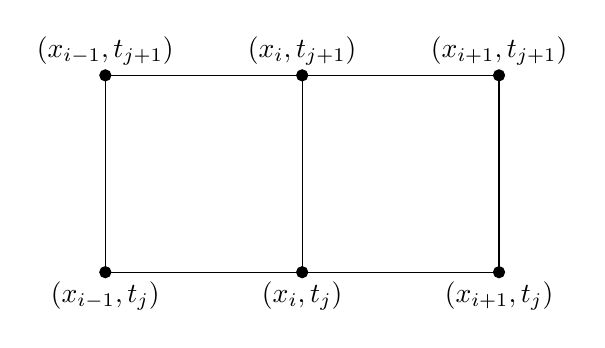
\begin{tikzpicture}
            \draw (-2.5, 0) -- (2.5, 0);
            \draw (-2.5, 2.5) -- (2.5, 2.5);
            \draw (-2.5, 0) -- (-2.5, 2.5);
            \draw (0, 0) -- (0, 2.5);
            \draw (2.5, 0) -- (2.5, 2.5);

            \filldraw[black] (-2.5, 0) circle(2pt) node[anchor=north] {$(x_{i - 1}, t_{j})$};
            \filldraw[black] (0, 0) circle(2pt) node[anchor=north] {$(x_{i}, t_{j})$};
            \filldraw[black] (2.5, 0) circle(2pt) node[anchor=north] {$(x_{i + 1}, t_{j})$};
            \filldraw[black] (-2.5, 2.5) circle(2pt) node[anchor=south] {$(x_{i - 1}, t_{j + 1})$};
            \filldraw[black] (0, 2.5) circle(2pt) node[anchor=south] {$(x_{i}, t_{j + 1})$};
            \filldraw[black] (2.5, 2.5) circle(2pt) node[anchor=south] {$(x_{i + 1}, t_{j + 1})$};
            
            % \draw (-2.5, 0) node[anchor=north] {$(x_{i - 1}, t_j)$} -- (2.5, 0) node[anchor=north] {$(x_{i + 1}, t_j)$};
            % \draw (-2.5, 2.5) node[anchor=north] {$(x_{i - 1}, t_{j + 1})$} -- (2.5, 2.5) node[anchor=north] {$(x_{i + 1}, t_{j + 1})$};
            % \draw (0, 0) -- (0, 2.5) node[anchor=south]{$(x_i, t_{j + 1})$};
            % \filldraw[black] (0, 0) circle(2pt) node[anchor=south west] {$(x_i, t_j)$};
            % \filldraw[black] (-2.5, 0) circle(2pt);
            % \filldraw[black] (2.5, 0) circle(2pt);
            % \filldraw[black] (0, 2.5) circle(2pt);
        \end{tikzpicture}
    \caption{Шеститочечный шаблон явной схемы}
    \label{fig:implicit_template}
\end{figure}
Идея неявных схем заключается в использовании шаблона, затрагивающего как значения функции на $j$--ом временном слое (который предполагается уже известным), так и на последующих слоях (значения функции на которых ещё не известны).
Так, однопараметрическое семейство неявных схем, зависящих от параметра $\sigma \in (0, 1]$ получается при аппроксимации дифференциального оператор на шеститочечном шаблоне (\seefigref{fig:implicit_template}), причём значения на \glqq верхнем\grqq и \glqq нижнем\grqq временных слоях берутся с весами $\sigma$ и $1 - \sigma$ соответственно.
Так, аппроксимация дифференциального оператора для одномерного уравнения с постоянными коэффициентами выглядит следующим образом:
\begin{multline*}
    L = \frac{\partial u}{\partial t} - \Delta u \mapsto 
    L_{h\tau} =\\
    = \frac{u_i^{j + 1} - u_i^j}{\tau} -
    \sigma\frac{u_{i + 1}^{j + 1} - 2u_i^{j + 1} + u_i^{j + 1}}{h^2}  -
    (1 - \sigma)\frac{u_{i + 1}^j - 2u_i^j + u_i^j}{h^2} + \phi_i^j,\\
    \phi_i^{j + 1} = f(x_i, t_{j + 1})
\end{multline*}
В многомерном случае можно задавать целый вектор $\sigma = (\sigma_1 \ldots \sigma_n)$:
\begin{multline*}
    L \mapsto 
    \frac{u_i^{j + 1} - u_i^j}{\tau} + \\
    + \sum\limits_{k = 1}^{n} \left[ 
        \sigma_k\frac{u_{i+}^{j + 1} - 2u_i^{j + 1} + u_{i-}^{j + 1}}{h_k^2} +
        (1 - \sigma_k) \frac{u_{i+}^j - 2u_i^j + u_{i-}^j}{h_k^2}
    \right] +\\
    + \phi_i^j,\text{ где }\\
    i_{\pm} = (i_1, \ldots, i_{k - 1}, i_k \pm 1, i_{k + 1}, \ldots, i_n)
\end{multline*}
Аналогично явной схеме, добавляя граничные и начальные условия, получаем замкнутую систему линейных уравнений.
Однако, в отличие от явной схемы, значения на новом временном слое $u^{j + 1}$ не выражаются явно через значения на предыдущем временном слое $u^{j}$, а получаются путём решения соответствующей системы линейных алгебраических уравнений $M u^{j + 1} = D$.
В одномерном случае матрица системы получается \emph{трёхдиагональной}:
\begin{equation*}
    M = \begin{pmatrix}
        B_1 & C_1 & 0 & 0 & 0 & 0 & 0\\
        A_2 & B_2 & C_2 & 0 & 0 & 0 & 0\\
        0 & A_3 & B_3 & C_3 & 0 & 0 & 0\\
        0 & 0 & A_4 & B_4 & C_4 & 0 & 0\\
        0 & 0 & 0 & \ddots & \ddots & \ddots & 0\\
        0 & 0 & 0 & 0 & A_{n-1} & B_{n-1} & C_{n-1}\\
        0 & 0 & 0 & 0 & 0 & A_{n} & B_{n}
    \end{pmatrix},
\end{equation*}
где 
\begin{align*}
    & A_i = -\sigma \tau\\
    & B_i = h^2 + 2\sigma \tau\\
    & C_i = -\sigma \tau\\
    & D_i = h^2 u_i^j + \tau (1 - \sigma) \left( 
        u_{i - 1}^j - 2u_i^j + u_{i + 1}^j
     \right) + \tau h^2 \phi_i^{j + 1}
\end{align*}
В таком случае существует эффективный алгоритм расчёта, именуемый \emph{методом прогонки}:
Сначала определяем $\alpha$ и $\beta$:
$$
    \begin{cases}
        \alpha_1 = -\frac{C_1}{B_1}, \\
        \beta_1 = \frac{D_1}{B_1}, \\
        \begin{aligned}
            & \alpha_i = -\frac{C_i}{B_i + A_i \cdot \alpha_{i-1}}\\
            & \beta_i = \frac{D_i - A_i \cdot \beta_{i-1}}{B_i + A_i \cdot \alpha_{i-1}}
        \end{aligned}, & i = 2, \ldots, n-1\\
        \beta_n = \frac{D_n - A_n \cdot \beta_{n-1}}{B_n + A_n \cdot \alpha_{n-1}}
    \end{cases}
$$
Затем по ним определяем неизвестные:
$$
    \begin{cases}
        x_n = \beta_n,\\
        x_i = \alpha_i \cdot x_{i+1} + \beta_i, & i = n-1, \ldots, 1
    \end{cases}
$$
Сложность такого алгоритма $O(N_x)$, что не уступает явной схеме.
Преимущества же неявной схемы в том, что для неё условия устойчивости принимает вид
\begin{equation*}
    \sigma \geqslant \frac{1}{2} - \frac{h^2}{4\tau}.
\end{equation*}
Из этого условия видно, что при $\sigma \ge 0.5$ схема безусловно устойчива, то есть устойчива вне зависимости от выбора шагов $h$ и $\tau$.

При значениях $\sigma \ne 0.5$ схема имеет порядок точности $O(h^2 + \tau)$, а при $\sigma = 0.5$ (так называемая \emph{схема Кранка-Николсона}) $O(h^2 + \tau^2)$, то есть больший, явная схема.

Недостатком такой схемы является отсутствие возможности распараллеливания.

В случае многомерной задачи дело обстоит хуже.
Получаемые системы линейных уравнений имеют более сложную матрицу (не трёхдиагональную). Для их решения пользуются в общем случае методом последовательного исключения переменных (методом Гаусса), который работает за $O(N^3)$, где $N \times N$~--- размерность матрицы.
Так, уже в двумерной задаче матрица будет размера $N_xN_y \times N_x N_y$, и расчёт будет проводиться заметно дольше, чем при расчёте явной схемой ($\sim O(N^2)$).
            % Локально-одномерные схемы
            \subsubsection{Локально-одномерные схемы}\label{sec:LOS}
            \newcommand{\valpha}{v_{(\alpha)}}

Итак, явные схемы обладают быстрой скоростью счёта ($\sim O(N^n)$), в то время как устойчивость таких систем достигается лишь при определённом выборе параметров сетки.
Неявные схемы безусловно устойчивы и имеют больший порядок точности, однако требуют решения системы $N^n$ уравнений, для чего требуется значительно больше вычислительной работы, чем для явной схемы \cite{ТихоновСамарский}.

Для сочетания лучших качеств явных (объём работы $\sim O(N^n)$) и неявных (безусловная устойчивость) схем было предложено несколько \emph{экономичных} схем.
Подбробнее об этом написано в \cite{СамарскийТеорияРазностныхСхем, peaceman1955numerical, douglas1955numerical, яненко1959одном, дьяконов1962разностные, самарский1962одном}.

\emph{Локально-одномерный метод} является универсальным, пригодным для решения квазилинейного уравнения теплопроводности в произвольной области $G$ любого числа измерений.
При использовании в работе блочных локально-адаптивных сеток \ref{sec:LAG} используется именно этот метод.
Также будут использоваться прямоугольные области, поэтому формулировка метода будет приведена для таковых.

Итак, рассматриваемую многомерную задачу Дирихле в цилиндре $\bar{Q}_T = \bar{G} \times [0, T]$, $\bar{G} = \prod\limits_{i=1}^{n} [0, L_i]$
\begin{equation*}
    \begin{aligned}
        &\left\{ 
            \begin{aligned}
                & u_t = \sum\limits_{\alpha = 1}^{p} \frac{\partial }{\partial x_{\alpha}} \left[ 
                    k_{\alpha}(u) \frac{\partial u}{\partial x_{\alpha}}
                 \right] + f, && (x, t) \in G \times (0, T]\\
                & \begin{aligned}
                    & u(x, t) = \mu_{-i}(x, t), && x_i = 0\\
                    & u(x, t) = \mu_{i}(x, t), && x_i = L_i
                \end{aligned}, && t \in [0, T)\\
                &u(x, 0) = u_0(x), && x \in \bar{G}
            \end{aligned}
        \right.\\
    \end{aligned}
\end{equation*}
заменяем \emph{цепочкой одномерных} задач \glqq вдоль каждого из напарвлений\grqq:
\begin{equation*}
    \begin{cases}
        \frac{1}{p} \frac{\partial v_{(\alpha)}}{\partial t} = \frac{\partial }{\partial x_{\alpha}} \left[ k_{\alpha}(v_{(\alpha)}) \frac{\partial v_{(\alpha)}}{\partial x_{\alpha}} \right] + f_{\alpha}, &
            x \in G, t \in \Delta_{\alpha} = \left( 
                t_{j + \frac{\alpha - 1}{p}}, 
                t_{j + \frac{\alpha}{p}}
            \right]\\
        \valpha(x, t_{j + \frac{\alpha - 1}{p}}) = v_{(\alpha - 1)}(x, t_{j + \frac{\alpha - 1}{p}}), & x \in G\\
        \valpha(x, t) = \mu_{-\alpha}(x, t), & x_{\alpha} = 0, t \in [t_{j + \frac{\alpha - 1}{p}}, t_{j + \frac{\alpha }{p}}]\\
        \valpha(x, t) = \mu_{\alpha}(x, t), & x_{\alpha} = L_{\alpha}, t \in [t_{j + \frac{\alpha - 1}{p}}, t_{j + \frac{\alpha }{p}}]\\
    \end{cases}
\end{equation*}
\begin{equation*}
    \begin{aligned}
        &\valpha(x, 0) = u_0(x)\\
        & v_{(1)}(x, t_j) = v_{(p)}(x, t_j)\\
        & u(x, t_{j + 1}) = v_{(p)}(x, t_{j + 1}).
    \end{aligned}
\end{equation*}
Каждая из одномерных задач решается неявной двухслойной шеститочечной схемой с весом $\sigma_{\alpha}$.
Пускай область $G$ дискретизуется сеткой $\omega_h$, имеющий вдоль каждого направления $N$ точек.
Для каждого значения $\alpha = 1, \ldots, p$ получается $N^{p - 1}$ задач. 
Каждая из них решается (методом прогодки как неявная одномерная схема) за $\sim O(N)$.
Таким образом, 



% \begin{equation*}
%     \frac{1}{p} \frac{\partial v_{(\alpha)}}{\partial t} =
%     \frac{\partial }{\partial x_{\alpha}} \left[ 
%                     k_{\alpha}(v_{(\alpha)}) \frac{\partial v_{(\alpha)}}{\partial x_{\alpha}} \right] + f_{\alpha},
% \end{equation*}
% \begin{equation*}
%     \text{где } t \in \Delta_{\alpha} = \left( 
%         t_{j + \frac{\alpha - 1}{p}}, 
%         t_{j + \frac{\alpha}{p}}
%     \right], \quad \alpha = 1, \ldots, p; \quad \sum_{\alpha = 1}^{p} f_{\alpha} = f
% \end{equation*}
% с граничными условиями:
% \begin{equation*}
%     \begin{cases}
%         \valpha(x, t) = \mu_{-\alpha}(x, t), & x_{\alpha} = 0, t \in \Delta_{\alpha}
%         \valpha(x, t) = \mu_{\alpha}(x, t), & x_{\alpha} = L_{\alpha}, t \in \Delta_{\alpha}
%     \end{cases}, \quad \alpha = 1, \ldots, p
% \end{equation*}
% и начальными условиями:
% \begin{equation*}
%     \begin{cases}
        
%     \end{cases}
% \end{equation*}

        % Программный код, примеры расчётов
        \subsection{Программный код, примеры расчётов}\label{sec:StaticCode}
        % \usemintedstyle[julia]{native}

Реализация вышеобозначенных разностных схем производилась с помощью языка программирования \texttt{Julia}\cite{bezanson2017julia}. 

В качестве иллюстрации простоты явной разностной схемы, в листинге \ref{listing:explicit_scheme} приведена её реализация для одномерного линейного уравнения теплопроводности.
\begin{listing}
    \begin{minted}[
        frame=lines,
        framesep=2mm,
        fontsize=\footnotesize,
        linenos=true,
        autogobble
        ]{julia}
    function explicit_scheme(f, u0, mu1, mu2, T, Nx, Nt)
        x = range(0, 1, length = Nx) # Точки секти по оси `x`
        t = range(0, T, length = Nt) # Точки сетки по оси `t`
        c = step(t) / step(x)^2 # Коэффициент Куранта
    
        u = zeros(Nx, Nt) # Матрица, хранящая решение разностной задачи
    
        u[:, 1] .= u0.(x) # Учёт начальных условий
        u[1, :] .= mu1.(t) # Учёт граничных условий на левом конце
        u[end, :] .= mu2.(t) # Учёт граничных условий на правом конце
    
        for j in 1:(Nt - 1) # Цикл по всем слоям
            for i in 2:(Nx - 1)
                u[i, j + 1] = u[i, j] + c * (u[i + 1, j] - 2 * u[i, j] + u[i - 1, j]) + 
                f(x[i], t[j])
            end
        end
    
        return u
    end
    \end{minted}
    \caption{Реализация явной схемы для уравнения $u_t = u_{xx} + f$}
    \label{listing:explicit_scheme}
\end{listing}
Заметим, что схема реализована для уравнения $u_t = u_{xx} + f$ на отрезке $x \in [0, 1]$, поскольку более общий вид уравнения $u_t = a^2 u_{xx} + \tilde{f}$ на отрезке $[a, b]$ сводится к первому линейной заменой $ t \mapsto \tilde{t} = \frac{(b - a)^2}{a^2} t, \quad x \mapsto \tilde{x} = \frac{x - a}{b - a}$.
Работоспособность программы была проверена на некоторых тестовых задачах \cite{горюнов2015методы}.
Так, для задачи
\begin{equation}\label{eq:task_1}
    \begin{cases}
        u_t = u_{xx} + f, & (x, t) \in (0, 1) \times (0, T]\\
        u(x, 0) = u_0(x), & x \in [0, 1]\\
        \begin{aligned}
            & \textstyle u(0, t) = \mu_1(t)\\
            & \textstyle u(1, t) = \mu_2(t)
        \end{aligned}, & t \in [0, T]
    \end{cases}
\end{equation}
расчитано решение для $T = 0.05$ для различного набора сеток с числом точек по оси времени $N_t = 25001$ и числом точек по оси $x$ в пределах от $N_x = 10$ до $N_x = 500$.
Заметим, что выбор такого, казалось, необоснованно большого числа точек по оси времени диктуется неустойчивостью явной разностной схемы: из условия устойчивости $\frac{\Delta t}{(\Delta x)^2} < \frac{1}{2}$ следует, что для $N_x = 500$ требуется $N_t > 25000$.
В таких простых, тестовых задачах такое соотношение ещё приемлемо, и современные компьютеры позволяют получить ршение достаточно быстро.
Однако в более сложных, многомерных задачах с резкими неоднородностями, требующими достаточно мелкого пространственного шага, это условие становится трудно выплонимым (такая точность по оси времени просто не требуется).
Явная схема была реализована только для линейного уравнения.
Как уже отмечалось выше, применения явной схемы нецелесообразно для квазилинейных уравнений.

\begin{figure}
    \centering
    \includegraphics{Разностные_схемы_на_статических_сетках/Программный_код_примеры_расчётов/explicit_scheme/problem_1_explicit_surface.pdf}
    \caption{Численное решение задачи \eqref{eq:task_1} для $N_x = 500$ и $N_t = 25\,001$}
    \label{fig:problem_1_explicit_surface}
\end{figure}
\begin{figure}
    \centering
    \includegraphics{Разностные_схемы_на_статических_сетках/Программный_код_примеры_расчётов/explicit_scheme/problem_1_analytic_surface.pdf}
    \caption{Аналитическое решение задачи \eqref{eq:task_1}}
    \label{fig:problem_1_analytic_surface}
\end{figure}
\begin{figure}
    \centering
    \includegraphics{Разностные_схемы_на_статических_сетках/Программный_код_примеры_расчётов/explicit_scheme/problem_1_explicit_error_surface.pdf}
    \caption{График локальной ошибки численного решения задачи \eqref{eq:task_1}}
    \label{fig:problem_1_explicit_error_surface}
\end{figure}
\begin{figure}
    \centering
    \includegraphics{Разностные_схемы_на_статических_сетках/Программный_код_примеры_расчётов/explicit_scheme/problem_1_explicit_time.pdf}
    \caption{График зависимости времени счёта от числа точек сетки $t(N_x)$ (в мс).}
    \label{fig:problem_1_explicit_time}
\end{figure}
На \figref{fig:problem_1_explicit_surface} представлено численное решение задачи как поверхность-график $u_h(x, t)$, полученное явной схемой для $N_x = 501$ и $N_t = 25001$.
На \figref{fig:problem_1_analytic_surface} представлен график зависимости аналитического решения задачи, полученного методом разделения переменных Фурье:
\begin{equation*}
    u(x, t) = \frac{1}{2}e^{-(3\pi)^2 t}\sin (3\pi x) - \frac{48}{\pi^2}\sum\limits_{m=1}^{\infty} \frac{m}{(9 - 4m^2)^2}e^{-(2\pi m)^2 t}\sin (2\pi m x)
\end{equation*}
Для точного сравнения также на \figref{fig:problem_1_explicit_error_surface} представлен график зависимости локальной ошибки $|u(x, t) - u_h(x, t)|$.
Для проверки утверждения о точности аппроксимации разностной схемы также построен график зависимости нормы разности аналитического и численного решения как функции от шага $h$ (\seefigref{fig:problem_1_explicit_time}).
Время выполнения рассчитывалось как среднее время от $\sim 100-200$ запусков программы для одних и тех же входных данных.

Реализация неявной схемы требует написания алгоритма прогонки для решения систем линейных уравнений с трёхдиагональной матрицей.
В листинге \ref{listing:tridiagonal_algorithm} представлен код алгоритма прогонки.
\begin{listing}
    \begin{minted}[
        frame=lines,
        framesep=2mm,
        fontsize=\footnotesize,
        linenos,
        autogobble
        ]{julia}
    # Оптимальный по памяти алгоритм прогонки в случае, если его нужно запускать много раз
    function tridiagonal_algorithm!(
            a::Vector{<:T}, b::Vector{<:T}, x::Vector{<:T},
            A::Vector{<:V}, B::Vector{<:V}, C::Vector{<:V}, D::Vector{<:V}
        ) where {T <: Number, V <: Number}
    
        a[1] = - C[1] / B[1]
        b[1] = D[1] / B[1]
        @inbounds for i=2:(length(B)-1)
            a[i] = - C[i] / (B[i] + A[i-1] * a[i-1])
            b[i] = (D[i] - A[i-1] * b[i-1]) / (B[i] + A[i-1] * a[i-1])
        end
        b[end] = (D[end] - A[end] * b[end-1]) / (B[end] + A[end] * a[end-1])
    
        # обратный ход
        x[end] = b[end]
        for i = length(B)-1:-1:1
            x[i] = a[i]*x[i+1] + b[i]
        end
    end
    \end{minted}
    \caption{Реализация алгоритма прогонки}
    \label{listing:tridiagonal_algorithm}
\end{listing}
Дополнительные переменные $\alpha, \beta, x$ передаются в функцию \texttt{tridiagonal\_algorithm} с целью экономии памяти.
Решение уравнения теплопроводности требует многократного выполнения алгоритма прогонки, поэтому общие временные переменные выделяются отдельно и сокращают количество ненужных аллокаций.
В листинге \ref{listing:implicit_scheme} приведена реализация неявной схемы для одномерного квазилинейного уравнения теплопроводности.
\begin{listing}
    \begin{minted}[
        frame=lines,
        framesep=2mm,
        fontsize=\footnotesize,
        linenos,
        autogobble
        ]{julia}
    function implicit_scheme(k, f, u0, mu1, mu2, T, Nx, Nt)
        x = range(0, 1, length = Nx) # Точки секти по оси `x`
        dx = step(x)
        t = range(0, T, length = Nt) # Точки сетки по оси `t`
        dt = step(t)
    
        u = zeros(Nx, Nt) # Матрица, хранящая решение разностной задачи
        u[:, 1] .= u0.(x) # Учёт начальных условий
        u[1, :] .= mu1.(t) # Учёт граничных условий на левом конце
        u[end, :] .= mu2.(t) # Учёт граничных условий на правом конце
    
        # Временные переменные для алгоритма прогонки
        A, C = (zeros(Nx) for i in 1:2)
        B, D, a, b, x = (zeros(Nx) for i in 1:5)
        B[1] = B[end] = 1
        C[1] = A[end] = 0
    
        for j in 1:(Nt - 1) # Цикл по временным слоям
            # Обновление коэффициентов тридиагональной матрицы
            D[1] = u[1, j + 1]
            D[end] = u[end, j + 1]
            for i = 2:(Nx - 1)
                A[i - 1] = -dt * k(0.5 * (u[i - 1, j] + u[i, j]))
                B[i] = dx^2 + dt * (
                    k(0.5 * (u[i, j] + u[i + 1, j])) +
                    k(0.5 * (u[i - 1, j] + u[i, j]))
                )
                C[i] = -dt * k(0.5 * (u[i, j] + u[i + 1, j]))
                D[i] = dx^2 * u[i, j] + dt * dx^2 * f(x[i], t[j])
            end
            tridiagonal_algorithm!(a, b, x, A, B, C, D) # Метод прогонки
            u[:, j + 1] .= x
        end
    
        return u
    end
    \end{minted}
    \caption{Реализация неявной схемы для уравнения $u_t = (ku_x)_x + f$}
    \label{listing:implicit_scheme}
\end{listing}
Работоспособность программы проверена на тех же тестовых задачах, что и для явной схемы.
Для проверки правильности учёта квазилинейности уравнения программа проверена на задаче, рассмотренной в статье~\cite{самарский1963примеры}:
\begin{equation*}
    \left\{
        \begin{aligned}
            &\frac{\partial u}{\partial t} = \frac{\partial }{\partial x}\left( \frac{1}{2}u^2 \frac{\partial u}{\partial x} \right), && (x, t) \in (0, 1)\times(0.1, 0.4)\\
            &\begin{aligned}
            &u(0, t) = 10\sqrt{t}\\
            &u(1, t) = 0
            \end{aligned}, && t\in [0.1, 0.4]\\
            &u(x, 0.1) = \left\{ \begin{aligned}
                &2\sqrt{5}\sqrt{0.5 - x}, && x \le 0.5\\
                & 0, && x\ge 0.5
            \end{aligned}\right. , && x \in [0, 1]
        \end{aligned}
    \right.
\end{equation*}
На графике (бла-бла) приведено численное решение, полученное неявной схемой на сетке с $N_x = 31$, $N_t = 50$ и аналитическое решение задачи:
\begin{equation*}
    u(x, t) = \left\{
        \begin{aligned}
            &\left[ \sigma c\varkappa_0^{-1} (ct + x_1 - x) \right]^{1/\sigma}, && x \le x_1 + ct\\
            &0, && x \ge x_1 + ct
        \end{aligned}
    \right.
\end{equation*}
где $\sigma = 2$, $\varkappa_0 = 0.5$, $x_1 = 0$, $c = 5$. 
Также на (бла-бла) представлен график зависимости локальной ошибки.
Видно, что основная погрешность сосредоточена в точках \emph{температурного фронта волны}: всюду, кроме некоторых точек около фронта, отклонение приближённого решения от аналитического не превосходит $2\cdot 10^{-3}$.

Однако для достижения такой же точности и \emph{вблизи особых точек} решения необходима достаточно мелкая сетка.
На (бла-бла) график решения и ошибки для $N_x = (\text{посчитать    })$.

Данный пример хорошо демонстрирует причину возникновения метода локально-адаптивных сеток.
Для получения точного решения вблизи особенности (фронта волны), необходима достаточно мелкая сетка $N \sim \text{число}$.
Напротив же, в остальных точках решение ведёт себя достаточно гладким и полчается точным уже при мелкой сетки $N \sim \text{число}$.
В одномерном случае с одной особой точкой эта ситуация может показаться не столь плохой.
Для многомерных же задач с большим числом особенностей и сильно меняющимися масштабами решения, где для получения заданной точности приходится использовать минимально необходимый шаг сетки во всей области сразу, число ненужных операций алгоритма значительно возрастает до недопустимых значений. 

В многомерных задачах, как уже отмечалось, получающиеся системы будут не трёхдиагональными, однако по-прежнему останутся достаточно разреженными (см. картинку и тут ссылка на картинку с spy matrix для 2d).
Реализация такой схемы заключается в прямом создании матрицы системы на каждом временном слое и решении с помощью общего алгоритма исключения переменных Гаусса.
\textbf{Вот тут вопрос: стоит ли в Приложении прикладывать листинг реализации этой схемы, и графики, демонстрирующие её работу и медлительность?}.

Локально-одномерная схема в сущности решает $N^{p - 1}$ одномерных задач, поэтому её реализация похожа на неявную схему, но с некоторыми отличиями.
В листинге (бла-бла) приведёт код этой схемы для двумерного квазилинейного уравнения теплопроводности (на случай больших размерностей код модифицируется очевидным образом (\textbf{стоит ли приводить для трёхмерного случая код в приложении?})).
Работоспособность проверена на задаче, рассмотренной в статье \cite{самарский1963примеры}:
\begin{equation*}
    \textstyle
    \begin{cases}
        u_t = (4u^4 u_x)_x + \left( \frac{1}{4} u^2 u_y \right)_y, \quad (x, y, t) \in (0, 30) \times (0, 20) \times (0, 50)\\
        u(x, y, 0) = 0,\\
        u(0, y, t) = \mu_{-1}(y, t) = \begin{cases}
            \scriptstyle\frac{1}{2}\sqrt{-1 + \sqrt{1 + 16(t - 2y)}}, & t > 2y\\
            \hfill 0, & t < 2y
        \end{cases}\\
        u(30, y, t) = \mu_1(y, t) = \begin{cases}
            \scriptstyle\frac{1}{2}\sqrt{-1 + \sqrt{1 + 16(t - 30 - 2y)}}, & t > 30 + 2y\\
            \hfill 0, & t < 30 + 2y
        \end{cases}\\
        u(x, 0, t) = \mu_{-2}(x, t) = \begin{cases}
            \scriptstyle\frac{1}{2}\sqrt{-1 + \sqrt{1 + 16(t - x)}}, & t > x\\
            \hfill 0, & t < x
        \end{cases}\\
        u(x, 20, t) = \mu_2(x, t) = \begin{cases}
            \scriptstyle\frac{1}{2}\sqrt{-1 + \sqrt{1 + 16(t - x - 40)}}, & t > x + 40\\
            \hfill 0, & t < x + 40
        \end{cases}
    \end{cases}
\end{equation*}
\textbf{Дальше только построение графиков и обсуждение результатов этих графиков, плавный переход к адаптивным сеткам}

\input{Разностные_схемы_на_статических_сетках/Программный_код_примеры_расчётов/test.tikz}
    
    % Теория блочных локально-адаптивных сеток
    \section{Теория блочных локально-адаптивных сеток}\label{sec:LAG}
    Большинство моделей классической физики, таких как гидрогазодинамика, описываются начально-краевыми задачами для дифференциальных уравнений в частных производных второго порядка\cite{ТихоновСамарский, ЛандауГидродинамика}.
Нахождение аналитического решения таких задач представляется возможным только в случае простых, канонических областей (таких как круг, шар, прямоугольник), простых начальных и граничных условий, а также в случае линейных уравнений, описывающих простые физические процессы.

На практике же часто возникают нелинейные задачи, поставленные в областях сложной формы.
Например, задача лазерного термоядерного синтеза (ЛТС), идя которой заключается в быстром нагреве и сжатии термоядерного топлива до температур и плотностей, необходимых для осуществления быстрого и эффективного протекания термоядерных реакций инерциально удерживаемой плазмы.
Процессы распространения тепла в такой системе будут описываться нелинейным уравнением теплопроводности.
Нелинейное уравнение теплопроводности также возникает в, например, задачах о самофокусировки световых пучков в нелинейных средах, эффекте $T$--слоя в низкотемпературной плазме, проблемы безударного сжатия; вообще с необходимостью в любой задаче, в которой присутствуют процессы самопроизвольного нарушения симметрии с понижением её степени \cite{ГалактионовКвазилинейное} 

Любой численный метод приближённого решения таких задач использует дискретизацию (то есть переход от бесконечномерного функционального пространства к конечномерному пространству).
Один из основных методов~--- \emph{метод конечных разностей}.
Его основа заключается в том, что исходная непрерывная задача в области $G \subset \mathbb{R}^n$ сводится к \emph{семейству разностных задач}~--- системам конечного числа линейных (в общем случае~--- нелинейных) уравнений на т.н. \emph{разностные функции}~--- функции, заданные на конечном числе точек (именуемое \emph{сеткой}), и принимающие значения (приближённые значения решения) на конечном числе точек.
Такие задачи решаются алгоритмически и тем самым могут быть программно реализованы на современных ЭВМ.
Более подробно метод описан в разделе~\ref{sec:MainDiffSchemes}.

Принципиальная возможность применения тех или иных алгоритмов основывается на вопросе об их сходимости, точности и устойчивости.
Так, в работе \cite{СамарскийТеорияРазностныхСхем} даётся обширное описание алгоритмов решения задач на \emph{статических} сетках, исследуются вопросы устойчивости и скорости сходимости.
Более подробное исследование тех же вопросов в случае \emph{неравномерных статических сеток} дан в работе \cite{СамарскийНеравномерныеСетки}.

Как уже отмечалось, в прикладных задачах приходится сталкиваться с квазилинейными уравнениями теплопроводности:
\begin{equation*}
    \frac{\partial u}{\partial t} =
    \sum\limits_{\alpha = 1}^{p} \frac{\partial }{\partial x_{\alpha}} \left[ 
        k_{\alpha}(u) \frac{\partial u}{\partial x_{\alpha}}
     \right]
\end{equation*}
Проблема использования \emph{статических} сеток, то есть сеток, не меняющихся на протяжении всего алгоритмического процесса поиска решения, связана со следующим обстоятельством.
В статьях \cite{ЗельдовичРазрывы, ЕщёРазрывы} показано, что одномерное уравнение теплопроводности в случае зависящего от температуры коэффициента теплопроводности имеет решения, производные которых разрывны в точках обращения в нуль решения $u(x, t)$, при этом поток тепла $k(u) \frac{\partial u}{\partial x}$~--- непрерывен, то есть существует фронт температуры, который, как показано в \cite{ЕщёЕщёРазрывы}, распространяется с конечной скоростью.
Эти \glqq проблемные точки решения\grqq оказываются сильно локализованными:
если для численного решения использовать достаточно грубые сетки, то основные ошибки в приближённом решении будут локализованны именно в окрестностях этих точек.
Конечно, можно использовать более мелкий шаг сетки и улучшить точность решения, ибо, как предсказывает теория \cite{СамарскийТеорияРазностныхСхем}, приближённое решение должно сходится к точному при стремлении шага сетки к нулю.

Однако даже на мощных вычислитльных системах расчёт сложных трёхмерных задач со сложной пространственной геометрией требует огромного числа точек сетки, что значительно увеличивает используемую память и расчётное время \cite{АфендиковЛАД}.
Более того, точность решения в области особенностей \emph{существенно} влияет на точность решения во всей остальной области.
Поэтому хотя бы для получения приемлемой кратины решения в целом на всей области без точного учёта особенностей неизбежно приходится сильно измельчать сетку.
Учитывая, что в подобластях гладкого поведения решения просто нет необходимости измельчать сетку настолько сильно, заключаем, что использование классических алгоритмов приводит к тому, что большая часть компьютерных вычислений производится напрасно.

Поэтому для данного класса гидродинамических проблем с локализованными особенностями разрабатывались специальные методы \emph{локально\hyp адаптивных сеток} (\emph{Adaptive mesh refinement}), учитывающие разномасштабное поведение решения.
Например, в работе \cite{СамарскийАдаптивные} предлагалось использовать адаптивную сетку, построение которой производится с помощью соответствующего преобразования координат.
Конкретный вид преобразования задаётся с помощью некоторой функции $Q$, вид которой определяется особенностями решения исследуемой задачи.
Т.к. вид функции $Q$ выбирался вручную в завимимости от конкретной задачи, этот метод не обладал достаточной автономностью.
Многие методы были основаны на геометрической адаптации рассчётных сеток, что, в свою очередь, приводит к трудностям реализации на ЭВМ, поскольку неструктурированные сетки порождают нерегулярный доступ к памяти.
С учётом современного развития массивно-параллельных архитектур процессоров с большим числом ядер, эффективность работы которых зависит в первую очередь от упорядоченности обращений в память, производительность методов с неструктурированными сетками оказывается неудовлетворительной.

\emph{Метод структурированных адаптивных сеток (Block-structured adaptive mesh refinement)} был представлен в работах \cite{berger1982adaptive, berger1989local} применительно к уравнениям гиперболического типа.
Преимущества метода в:
\begin{itemize}
    \item использовании простых прямоугольных областей определённого размещения, удобных для реализации на компьютере
    \item возможности использования архитектуры параллельных вычислений
    \item использовании точно таких же разностных схем, как и для статических декартовых сеток (с некоторыми алгоритмическими модификациями)
\end{itemize}.

\textbf{Целью данной работы} является изучение метода стрктурированных декартовых локально-адаптивных сеток применительно к задачам для уравнения теплопроводности, программная реализация данного метода, сравнение со статическими аналогами.

В разделе \ref{sec:MainDiffSchemes} вводятся основные математические формулировки разностных задач.
В разделе \ref{sec:StaticGrid} описываются алгоритмы решения задач на статических сетках (которые в последствии непосредственно используются при решении методом адаптивных сеток), приводятся примеры решения модельных задач.
В разделе \ref{sec:LAG} приводится описание метода, программной реализации и результатов решения модельных задач.
        
        \subsection{Топология сетки}
        Далее для простоты и определённости рассматривается двумерный случай.
На случай больших размерностей все определения непосредственно переносятся.

Адаптивная сетка состоит из последовательности \emph{уровней} $l = 1, 2, \ldots, l_{\text{max}}$.
Каждый уровень представляет из себя набор прямоугольных областей $G_{l, m}$, где $l$ нумернует уровень, $m$~--- номер прямоугольной области (блока) на данном уровне.
Считаем, что на уровне $l$ находится $M_l$ блоков.
Общее множество, занимаемое уровнем $l$ есть
\begin{equation*}
    G_{l} = \bigcup_{m = 1}^{M_{l}} G_{l, m}
\end{equation*}
Уровень $l = 1$ будем называть основным, главным или корневым.
Этот уровень считаем состоящим из $M_{1} = 1$ прямоугольной области $[0, L_x] \times [0, L_y]$, которая дискретизуется равномерной сеткой:
\begin{equation*}
    \omega_{1, 1} = \left\{ (x_i, y_j) \mid x_i = (i - 1) * h_x, y_j = (j - 1) * h_y, i = 1, \ldots, N_x, j = 1, \ldots, N_y \right\}.
\end{equation*}
Каждый последующий уровень дискретизуется более мелкой сеткой, а именно шаг и по оси $x$ и по оси $y$ при переходе с уровня $l - 1$ на уровень $l$ уменьшается в $r_{l}$ раз.
Чаще всего рассматривают $r_{l} = 2, 4$.
В этой работе для определённости и простоты реализации расматривается фиксированный $r_l = 2 \quad \forall l > 1$.
Также на такую иерархию накладывается ограничение \emph{корректно-вложенных} уровней:
\begin{equation*}
    G_{l} \cap G_{l - 1} = G_{l}
\end{equation*}
то есть уровень $l + 1$ целиком должен лежать в уровне $l$.
(В ячеечном формализме это утверждение может быть сформулировано следующим образом: в окрестности каждой ячейки не должно быть ячеек, отличающихся от неё по размерам более чем в два раза).
Множество точек на каждом блоке нумеруется (локально) индексной системой координат $(i, j)$.
Таким образом, уровень $l$ должен хранить положения блоков $G_{l, 1}, \ldots, G_{l, M_{l}}$ в индексных координатах надблока уровня $l - 1$.
Пример корректной блочно-стурктурированной декартовой сетки приведён на \figref{fig:example_BSG}
\begin{figure}
    \centering
    \includegraphics{Теория_блочных_локально_адаптивных_сеток/Топология_сетки/grid_topology.pdf}
    \caption{Пример корректной блочно-структурированной декартовой сетки}
    \label{fig:example_BSG}
\end{figure}


        \subsection{Численное обновление}
        Пускай известно решение на временном слое $j$, то есть известно $u_{i, k}^{j} \quad \forall i, k$.
Решение на новом временном слое ищется постепенно, от груого к мелкому, используя какую-либо ранее расмотренную разностную схему для статических сеток.
Как уже отмечалось, использование явной схемы нецелесообразно ввиду отсутствия устойчивости.
В работах \cite{жуков2015численное} используется явно-итерационная схема ЛИ-М, опирающаяся на оптимальные свойства многочлена Чебышева специальной конструкции, о чём подробнее можно прочитать в \cite{жуков2010явных, жуков2015решении, жуков2014параллельный}
Предпочтение было отдано локально-одномерной схеме, ввиду всех её преимуществ, описанных ранее в разделе \ref{sec:LOS}

Сначала обновляется решение на самой крупной сетке, то есть на уровне $l$.
Затем ищется решение на более точной сетке. 
Так как в общем случае $\partial G_l \not\subset \partial G_1$, то сразу не понятно, как учитывать граничные условия в схеме обновления решения.

        \subsection{Граничные условия}
        Поступают следующим образом: при решение на уровне $l$, в качестве граничных значений для обновления $t_j \mapsto t_{j + 1}$ берутся уже найденные приблежённые значения на слое $t_{j + 1}$ на уровне $l - 1$ (то есть на предыдущем уровне).
Значение в точках $\partial \omega_l \cup \omega_{l - 1} \not\subset \omega_{l + 1}$ задаётся путём линейной интерполяции со значений в точках $\partial \omega_l \cup \omega_{l - 1} \subset \omega_{l + 1}$.
Рисунок \ref{fig:linear_interpolation} описывает вышескзаанное.
\begin{figure}[h]
    \centering
    \begin{tikzpicture}
        \filldraw (0, 0) circle (2pt);
        \filldraw(2, 0) circle (2pt);
        \filldraw(3, 0) circle (2pt);
        \filldraw(4, 0) circle (2pt);
        \filldraw(6, 0) circle (2pt);

        \filldraw (0, 2) circle (2pt);
        \filldraw(2, 2) circle (2pt) node[anchor=south east] {$A$};
        \filldraw(3, 2) circle (2pt) node[anchor=north] {$D$};
        \filldraw(4, 2) circle (2pt) node[anchor=south west] {$B$};
        \filldraw(6, 2) circle (2pt);

        \filldraw(2, 1) circle (2pt);
        \filldraw(3, 1) circle (2pt);
        \filldraw(4, 1) circle (2pt);

        \draw (2, 2) arc (150:30:1.15);

        \draw [-{Stealth[length=3mm, width=2mm]}] (3, 3.2) node[anchor=west]{$u_l(D) =\frac{1}{2}(u_{l - 1}(A) + u_{l - 1}(B))$} -- (3, 2.2);
    \end{tikzpicture}
    \caption{Интерполяция с грубой сетки}
    \label{fig:linear_interpolation}
\end{figure}
Так, точки $A$, $B$ принадлежат уровню $l - 1$.
Точки $C$, $D$, $E$ принаждлежат уровню $l$.
Точки $C$ и $E$ совпадают с точками $A$ и $B$, и решение в них задаётся с уровня $l - 1$, а значение в \glqq промежуточной\grqq точке $D$ задаётся линейной интерполяцией значений с точек $A$ и $B$:
\begin{equation*}
    u_l(D) = \frac{u_{l - 1}(A) + u_{l - 1}(B)}{2}
\end{equation*}
Для большей точности расчёта помимо измелчение пространственной сетки происходит и измельчение временной сетке, а именно:
\begin{equation*}
    \frac{\Delta x_{l}}{\Delta x_{l - 1}} = \frac{\Delta t_{l}}{\Delta t_{l - 1}}.
\end{equation*}
Это позволяет, например, избежать появлений неустойчивости в случае использования явной схемы.

        \subsection{Данные на сетке}
        Очевидно использовать обыкновенные многомерные массивы для хранения данных численного решения на таких блочных сетках невозможно, а точнее, неэффективно.
Задача отыскания наиболее удобного и оптимального формата хранения данных на сетках с локальной адаптацией~--- одна из ключевых.
Существует несколько методов.
Так, в \cite{АфендиковЛАД} используются древовидные структуры (четвертичные и восьмиричные деревья).
В этой работе для хранения данных используется двусвязный список.
Каждый уровень \texttt{Level} описывается следующей структурой (несущественные в идеологическом плане тонкости реализации опускаются в коде):
\begin{minted}{julia}
struct Level
    level_number::Int # номер уровня в иерархии уровней
    sublevel::Union{Nothing, Level} # подуровень
    suplevel::Union{Nothing, Level} # надуровень

    blocks::Vector{Block} # массив блоков сеток
    M::Int # число блоков сетки

    t_curr::Real # Текущее время на уровне
    delta_t::Real # Временной шаг уровня
end
\end{minted}
Поля \texttt{sublevel} и \texttt{suplevel} имеют тип \texttt{Union\{Nothing, Level\}}, что означает, что эти переменные могут быть как типа \texttt{Level} (то есть быть ссылкой на под- или над- уровни соответственно), так и типа \texttt{Nothing} (то есть не существовать, а значит, уровень не имеет подуровня (последний уровень измельчения) или надуровня (уровень является корневым)).
Тип блок имеет вид:
\begin{minted}{julia}
struct Block
    spacial_grid::UniformGrid # Сетка

    # Координаты `((x1, x2), (y1, y2))` положения блока в
    # надблоке (в индексных координатах надблока)
    supblock_position::Tuple{Tuple{Int, Int}, Tuple{Int, Int}}
    
    u::Matrix{Real} # Решение
end
\end{minted}
\texttt{UniformGrid}~--- удобное представление равномерной сетки, которая использовалась ранее.

        \subsection{Рекурсивный алгоритм}
        Основной алгоритм записывается достаточно просто после того, как учтено, каким образом хранятся данные, и реализована схема для равномерных сеток.
Основные детали алгоритма могут быть записаны в следующем виде:
\begin{minted}{julia}
function solve(problem::HeatProblem, grid_params)
    # учёт начальных условий
    initial_conditions!(problem, grid_params)

    # Идём по всем временным слоям
    for j in 1:(grid_params.Nt - 1)
        levels[j + 1] = deepcopy(levels[j])
        advance_level!(problem, levels[j + 1])
    end
end
\end{minted}
Функция \texttt{initial\_conditions!} устанавливает значение в момент времени $t_1$, то есть для каждой точки $(x, y)$ блочной сетки, для каждого уровня считается значение $u_0(x, y)$.

Затем выполняется послойное обновление решения: зная $u(x, y, t_j)$ для любых $(x, y) \in \omega$ (то есть зная решение на временном слое $t_j$), находится решение на следующем временном слое $t_{j + 1}$ с помощью функции \texttt{advance\_level!}.
Эта функция вызывается на коневом уровне $l = 1$, а затем рекурсивно на всех подуровнях.
Это иллюстрирует листинг:
\begin{minted}{julia}
function advance_level!(problem::HeatProblem, level::Level)
    for i in 1:r_l # r_l --- refinement ratio
        numerical_update_u(problem, level)
        if has_sublevel(level)
            advance_level!(problem, level.sublevel)
        end
        level.t_curr += level.delta_t
    end
    interpolate_fine_to_coarse(level)
end
\end{minted}
С помощью локально-одномерной схемы функция \texttt{numerical\_update\_u} обновляет решение на уровне \texttt{level}, и если уровень имеет подуровень (\texttt{has\_sublevel(level) == true}), выполняется обновление на этом подуровне.
Причём, обновление на подуровне происходит $r_l$ раз, то есть соответствует \eqref{eq:frac_time_step}.
В нашем случае $r_l = 2 \quad \forall l > 1$, что значит, что переход $t_j \mapsto t_{j + 1}$ от старого временного слоя к новому на уровне $l$ будет осуществляться за $2^{l - 1}$ шагов.

Отметим ещё одну особенно важную часть алгоритма, требующую отдельного подробного исследования, и поэтому не рассмотренную в работе: перестройку сетки с учётом особенностей решения.
После того, как получено решение на новом временном слое, необходимо проанализировать полученное решение и найти новое положение особенностей решения.
Запускается так называемый процесс индикации перестройки (refinement indication).
Индикатор оценивает текущую точность численного решения и отмечает области сетки, в которых нужна большая/меньшая точность.
Было предложено достаточно большое количество индикаторов (например, в работах \cite{berger1989local, berger1982adaptive, lohner1987adaptive}).
После того, как были отмечены точки, в которых требуется большая точность, запускается процесс перестройки сетки (regridding).
Задача состоит в том, чтобы покрыть отмеченные точки блоками мелкой сетки таким образом, чтобы неотмеченных точек, попадающих в мелкую сетку было как можно меньше (то есть покрытие особенностей решения оптимальным образом, так называемый clustering algorithm).
Также, как и с индикаторами, существует множество различных алгоритмов кластеризации, с некоторыми вариантами можно ознакомиться в \cite{berger1989local, deiterding2011block}.

        \subsection{Результаты моделирования}
        Тестирование реализованного алгоритма на блочно-структурированных сетках проводилось на задаче \eqref{eq:problem_3}.
Так как проводилось исследование работоспособности именно блочности сетки, а не её динамической адаптации, был выбран отрезок времени $t \in [40, 42]$.
На \figref{fig:block_structured_grid} представлена сетка, на которой проивоздился расчёт.
\begin{figure}[h]
    \centering
    \includegraphics[width=\textwidth, height=\textheight, keepaspectratio]{Теория_блочных_локально_адаптивных_сеток/Результаты_моделирования/grid.pdf}
    \caption{Блочно-структурированная сетка, учитывающая особенность решения}
    \label{fig:block_structured_grid}
\end{figure}
Из рисунка видно, что самая грубая сетка соответствует выбору числа точек $N_x = 41$ и $N_y = 21$.
График ошибок численного решения, полученного только на грубой сетке, приведён на \figref{fig:coarse_errors}
\begin{figure}
    \centering
    \includegraphics[width=\textwidth, height=\textheight, keepaspectratio]{Теория_блочных_локально_адаптивных_сеток/Результаты_моделирования/errors_before.pdf}
    \caption{График ошибок численного решения на грубой сетке $N_x = 41, N_y = 21$.}
    \label{fig:coarse_errors}
\end{figure}
График ошибок численного решения, полученного при использовании описанного выше алгоритма на стрктурированной сетке приведён на \figref{fig:structured_errors}
\begin{figure}
    \centering
    \includegraphics[width=\textwidth, height=\textheight, keepaspectratio]{Теория_блочных_локально_адаптивных_сеток/Результаты_моделирования/errors_after.pdf}
    \caption{График ошибок численного решения на блочно-структурированной сетке с тремя уровнями измельчения}
    \label{fig:structured_errors}
\end{figure}
Из него непосредственно видно, что ошибка вблизи особенностей заметно уменьшилась.
Также видно большее \glqq размытие\grqq окрестности особенности решения.
Это указывает на то, что такая сетка \glqq размывает\grqq пики вблизи разрывов, делая погрешность решения более равномерной по всей области (что и соответствует тому, что мы находим решение с заданной точностью во всей области сразу).
Также сравнивалось время, затраченное на расчёт на такой блочно-структурированной сетке и на равномерной сетке, соответствующей самому мелкому разбиению из блочно-структурированной сетки: производительность первой программы оказалась $\approx$ в 10 раз выше.
Таким образом, показаны основные достоинства реализованного алгоритма.

\begin{wrapfigure}{r}{0.3\textwidth}
    \begin{center}
        \includegraphics[width=0.25\textwidth, height=0.4\textheight, keepaspectratio]{Теория_блочных_локально_адаптивных_сеток/Результаты_моделирования/artifact.png}
    \end{center}
    \caption{Недочёты алгоритма}
    \label{fig:artifacts}
\end{wrapfigure}
В процессе разработки и тестирования были найдены ошибки и недочёты программы, а именно, при достаточно большом количестве блоков и при их небольшом размере возможно возникновение так называемых артефактов решения (\seefigref{fig:artifacts}), появляющихся на стыках двух блоков одного уровня.
Скорее всего, данная особенность возникает из-за не совсем корректного учёта синхронизации данных на двух блоках.
Точная причина и пути её устранения ещё подлежат дальнейшему анализу.


    % Заключение
    \newpage
    \section{Заключение}
    В работе был проведён подробный анализ некоторых разностных схем численного решения уравнения теплопроводности, исследование их устойчивости, точности и скорости счёта, а именно:
\begin{itemize}
    \item явной разностной схемы
    \item однопараметрического семейства неявных разностных схем, в том числе чисто неявной схемы для квазилинейного уравнения
    \item локально-одномерной схемы
\end{itemize}
Проделанный анализ сопровождался проведением большого количества численных расчётов с помощью написаного программного обеспечения, реализующего все вышеперечисленные разностные схемы и позволяющего решать задачу Дирихле для одномерного и многомерного уравнения теплопроводности с произвольными граничными и начальными данными, а также позволяющего демонстрировать точность и скорость счёта разностных схем.
Показаны преимущества и недостатки использования равномерных статических сеток на конкретных примерах из различных статей.

Сделан обзор литературы, посвещённой методу блочно-структурированных локально-адаптивных сеток (block-structured adaptive mesh refinement), разработан алгоритм решения квазилинейного уравнения теплопроводности на блочно-структурированной сетке с использованием локально-одномерной схемы для обеспечения устойчивости метода, который реализован в виде программного кода.
Исследована работоспособность алгоритма, показаны преимущества использования локального измельчения сетки.

Разработка численных методов локальной-адаптации для решения прикладных задач является актуальной и неослабевающей научной проблемой, привлекающей как исследователей из области вычислительной математики, так и физиков-экспериментаторов благодаря возможности поставить дорогостоящие эксперименты виртуально на компьютере.
В настоящее время проблема полностью не решена и в научном мире ведутся активные исследования на эту тему.

В будущем планируется разработка программного обеспечения с переносом функционала, реализованного в \cite{ranocha2022adaptive, schlottkelakemper2021purely, schlottkelakemper2020trixi} для гиперболических проблем, на случай параболических уравнений, областей произвольной формы и возможности распараллеливания программы.

    % Список Литературы
    \newpage
    \renewcommand{\refname}{Список литературы}
    \printbibliography
    \addcontentsline{toc}{section}{\refname}
\end{document}